\documentclass[../main.tex]{subfiles}
\begin{document}
\lstset{language=Matlab}

\section{Problem 2}
\label{cha:problem-2}

\subsection{Introduction}
\label{sec:introduction}
In this problem, we will implement a program that calculates stress
response of a planar sheet of non-linear hyperelastic material
subjected to a given deformation.  We have been given a compressible
neo-Hookean hyperelastic model which has strain energy defined as
\begin{align}
  \label{eq:w}
  w(\mathbf{C}) = \frac{\lambda_0}{2}\ln^2(J) - 
  \mu_0\ln(J)+\frac{\mu_0}{2}(I_1-3)
\end{align}
where
\begin{align*}
  I_1 = tr(\mathbf{C}) = C_{kk},\quad J =
  det(\mathbf{F}),\quad \mathbf{C}=\mathbf{F}^T\mathbf{F}.
\end{align*}
By definition, first Piola-Kirchhoff stress tensor is given as
\begin{align*}
  P_{iJ} &=\frac{\partial
           w(\mathbf{C})}{\partial F_{iJ}}\\
         &=
           \left(\lambda_0\ln(J)-\mu_0\right)\frac{\partial}{\partial
           F_{iJ}}(\ln(J)) +
           \frac{\mu_0}{2}\left(\frac{\partial}
           {\partial F_{iJ}}(F_{lK}F_{lK})\right)\\
\end{align*}
Now, we can simplify above equation using following two results
\begin{align*}
  \frac{\partial}{\partial F_{iJ}}(\ln(J))&= \frac{1}{J}\frac{det(\mathbf{F})}
                                            {\partial F_{iJ}}\\
                                          &=  \frac{1}{J}JF^{-1}_{Ji}\\
                                          &= F^{-1}_{Ji}\\
  \frac{\partial}{\partial F_{iJ}}(F_{lK}F_{lK}) &=2F_{lK}\delta_{li}\delta_{KJ}\\
                                          &= 2F_{iJ}
\end{align*}
Thus we get,
\begin{align}
  \label{eq:P}
  \boxed{P_{iJ}=(\lambda_0\ln(J)-\mu_0)F^{-1}_{Ji}+\mu_0F_{iJ}}
\end{align}

The tangent modulus is a derivative of first Piola-Kirchhoff stress
tensor with respect to the deformation gradient. Using the last two
quations we can calculate the derivative as follows
\begin{align*}
  C_{iJkL}&=\frac{\partial P_{iJ}}{\partial F_{kL}}\\
          &= \left(\lambda_0\ln(J) - \mu_0\right)\frac{\partial F^{-1}_{Ji}}{\partial F_{kL}} + \frac{\lambda_0}{J}\left(\frac{\partial det(\mathbf{F})}{\partial F_{kL}}\right)F^{-1}_{Ji} + \mu_0\delta_{ki}\delta_{LJ}\\
\end{align*}
We can simplify this equation using the result
\begin{align*}
  \frac{\partial F^{-1}_{Ji}}{\partial F_{kL}} = -F^{-1}_{Jk}F^{-1}_{Li}
\end{align*}
\begin{align}
  \label{eq:C}
  \boxed{C_{iJkL}=\lambda_0F^{-1}_{Ji}F^{-1}_{Lk} + \mu_0\delta_{ik}\delta_{JL}-(\lambda_0\ln(J) - \mu_0)F^{-1}_{Jk}F^{-1}_{Li}}
\end{align}

Equations \ref{eq:w}, \ref{eq:P} and \ref{eq:C} give 3-D behavior of a
compressible neo-Hookean material. Next, we will adapt these equations
for 2-D \textit{plane stress} case. Consider a planar sheet of
compressible neo-Hookean material lying in the 1-2 plane of the lab
frame. Thus, the normal to the surface is $\bm{N} = \bm{E}_3$.  A
planar deformation implies there should not be any shearing in the
3-direction. But in response to the in-plane stretching we can expect
a compression in the 3-direction. Thus, our deformation gradient can
be assumed to look like
\begin{align*}
  [F_{iJ}] =
  \begin{pmatrix}
    F_{11} & F_{12} & 0\\
    F_{21} & F_{22} & 0\\
    0 & 0 & \lambda
  \end{pmatrix}
\end{align*}
In order that there is no stress in the 3-direction, we should set the
component of traction vector in that direction to be zero in the
deformed configuration. But because of planar stress we also expect
the surface normal in deformed and reference configuration to be in
the same direction i.e. $\bm{n} = \bm{N}$. We also assume that the
traction vectors are same in the reference and deformed
configuration. Hence, we can write
\begin{align}
  \label{eq:planeStress}
  T_N = \bm{N}\cdot P\bm{N} = P_{33}(F_{\alpha\beta},\lambda) = 0 \quad \alpha,\beta\in{1,2}
\end{align}
In general, $\mathbf{P}$ is a function of components of
$\mathbf{F}$. Hence, for plane stress we can write
$P_{33}(F_{\alpha\beta},\lambda))$. We need to solve for $\lambda$
using the known values of $F_{\alpha\beta}$. This will be discussed in
next section.

Let us define the strain energy density, first Piola-Kirchhoff stress
and the tangent modulus for plane-stress condition as follows
\begin{align*}
  w^{(2D)}(\mathbf{F}) &\equiv w^{(3D)}(F_{\alpha\beta},\lambda(F_{\alpha\beta}))\\
  P^{(2D)}_{\alpha\beta}(\mathbf{F})&\equiv \frac{\partial}{\partial F_{\alpha\beta}}(w^{(2d)})\\
                       &= \frac{\partial w^{(3D)}}{\partial F_{\alpha\beta}} +\cancelto{P_{33}=0}{\frac{\partial w}{\partial \lambda}}\frac{\partial \lambda}{\partial F_{\alpha\beta}}\\
                       &= \frac{\partial w^{(3D)}}{\partial F_{\alpha\beta}}\\
  C^{(2D)}_{\alpha\beta\gamma\delta}(\mathbf{F})&\equiv \frac{\partial}{\partial F_{\gamma\delta}}\left(P^{(2D)}_{\alpha\beta}\right)\\
                       &=\frac{\partial P_{\alpha\beta}}{\partial F_{\gamma\delta}} + \frac{\partial P_{\alpha\beta}}{\partial F_{33}}\frac{\partial\lambda}{\partial F_{\gamma\delta}}
\end{align*}
Using plane strain constraint we find that
\begin{align*}
  P_{33}(F_{\alpha\beta},\lambda)&=0\\
  dP_{33} = \frac{\partial P_{33}}{\partial F_{\alpha\beta}}dF_{\alpha\beta} + \frac{\partial P_{33}}{\partial F_{33}}d\lambda &= 0\\
  \implies \quad C_{33\alpha\beta}dF_{\alpha\beta}+C_{3333}d\lambda &=0\\
  C_{33\alpha\beta}dF_{\alpha\beta}+C_{3333}\frac{\partial\lambda}{\partial F_{\alpha\beta}}dF_{\alpha\beta} &=0\\
  \left(C_{33\alpha\beta}+C_{3333}\frac{\partial\lambda}{\partial F_{\alpha\beta}}\right) &=0\\
  \implies\quad\boxed{\frac{\partial\lambda}{\partial F_{\alpha\beta}} = -\frac{C_{33\alpha\beta}}{C_{3333}}}
\end{align*}
Therefore, the 2-D tangent modulus is given as
\begin{align*}
  \boxed{C^{(2D)}_{\alpha\beta\gamma\delta} = C_{\alpha\beta\gamma\delta} - C_{\alpha\beta33}C_{33\gamma\delta}\left(C_{3333}\right)^{-1}}
\end{align*}
Thus we have obtained all theoretical results required to solve our
problem. Now, let's look at some numerical aspects of the solution.
\subsection{Formulation of Numerical Methods}

\subsubsection{Neo-Hookean function}
First of all, we will implement a function that takes as input a valid
deformation gradient $\mathbf{F}$ and material constants, $\lambda_0$
and $\mu_0$, as input and returns the strain engergy density $w$,
first Piola-Kirchhoff stress tensor $\mathbf{P}$ and the tangent
modulus $C_{iJkL}$ as output using the analytical results derived in
the introduction. We use multidimensional array to store the fourth
order tensor, $C_{iJkL}$. We also implemented a small function
\textit{kronDel()} that takes two indices $i$ and $j$ as input and
returns $1$ if $i=j$ and $0$ otherwise.
\subsubsection{Generating valid arbitrary deformation gradient}
We generate a random matrix $\mathbf{H}$ of size $3\times 3$. A valid
deformation gradient should have $J = det(\mathbf{F}) > 0$. We can
ensure this if $\mathbf{F}$ is a positive definite matrix. Hence, we
construct the deformation gradient as $\mathbf{F} = \mathbf{HH}^T$
\subsubsection{Consistency test}
\label{sec:consistency}
As we saw in the introduction, $\mathbf{P}$ is derivative of $w$ with
respect to $\mathbf{F}$ and $C_{iJkL}$ is derivative of $P_{iJ}$ with
respect to $F_{kL}$ for any valid deformation. We also derived the
analytical expressions for $P_{iJ}$ and $C_{iJkL}$. We can validate
our code, by testing if numerical differentiation of $w$ and
$\mathbf{P}$ tallies with the analytical equations for $\mathbf{P}$
and $C_{iJkL}$ respectively. This is called consistency test.  We will
use 3-point finite difference scheme for numerical differentiation. As
per this scheme, if $h$ is small perturbation in the value $x$, the
derivative of function $f(x)$ is given as
\begin{align*}
  f'(x) \approx \frac{f(x+h)-f(x-h)}{2h} = f'_h(x)
\end{align*}
This method has error $\mathcal{O}(h^2)$.
\begin{align*}
  \text{erro}r = |f'_h(x) - f'(x)| &= Kh^2\\
  \log(\text(erro)r) &= \log(K) + 2\log(h)\\
\end{align*}
where $K$ is some constant. So on a log-log plot of $\text{error}$ vs
$h$ should give us a straight line of slope $2$.  For our problem, the
numerical derivatives are given as follows:
\begin{align*}
  P^{(h)}_{iJ}(F_{iJ}) &= \frac{w(F_{iJ}+h) - w(F_{iJ}-h)}{2h}\\
  C^{(h)}_{iJkL}(F_{kL})&=\frac{P_{iJ}(F_{kL}+h) - P_{iJ}(F_{kL}-h)}{2h}\\
\end{align*}
\subsubsection{Generating a random rotation matrix}
We used Rodrigues equation to otbain rotation matrix $\mathbf{Q}$ for
rotation around a randomly generated axis $\mathbf{v}$ by a random
angle $\theta$. We check that the rotation matrix actually belongs to
$SO^3$ by checking if $det(\mathbf{Q}) = 1$ and
$\mathbf{Q}^{-1} =\mathbf{Q}^T $
\begin{lstlisting}[style = Matlab-editor]
  v = rand(3,1); n = v/norm(v); theta = rand(1)*pi; n_hat =
  [0,-n(3),n(2); n(3),0,-n(1);-n(2),n(1),0]; Q = eye(3) +
  sin(theta)*n_hat + (1- cos(theta))*(n*n' - eye(3)); tol = 10^-7;

  % Check if Q belongs to SO3
  if (abs(det(Q)-1) > tol || norm(abs(inv(Q) - Q')) > tol) error('Q
  does not belong to SO3.\n'); end
\end{lstlisting}

\subsubsection{Material Frame Indifference test}
\label{sec:mfi}
A valid constitutive material model must satisfy material frame
indifference, that is, the stress response should be independent of
the coordinate representation used in calculation. One way to check
this is to compare $w$, $\mathbf{P}$ and $C_{iJkL}$ obtained for a
deformation gradient $\mathbf{F}$ with the same quantities calculated
for $\mathbf{F}$ in a rigidly rotated co-ordinate
system. Theoretically, the two set of quantities should compare as
follows.
\begin{align*}
  w(\mathbf{QF}) &= w(\mathbf{F})\\
  \mathbf{P}(\mathbf{QF}) &= \mathbf{Q}\mathbf{P}(\mathbf{F})\\
  C_{iJkL}(\mathbf{QF}) &= Q_{im}Q_{kn}C_{mJnL}(\mathbf{F})
\end{align*}

\subsubsection{Isotropy test}
\label{sec:isotropy}
Compressible neo-Hookean model is designed to be isotropic. The
stress-response of the material should not change arbitrarily by just
a rigid rotation of the deformation. Rather, a rotated deformation
should yield quantities that are related to their counterparts for
original deformation as follows
\begin{align*}
  w(\mathbf{FQ}) &= w(\mathbf{F})\\
  \mathbf{P}(\mathbf{FQ}) &= \mathbf{P}(\mathbf{F})\mathbf{Q}\\
  C_{iJkL}(\mathbf{QF}) &= Q_{MJ}Q_{NL}C_{iMkN}(\mathbf{F})
\end{align*}

\subsubsection{Newton-Raphson method}
\label{sec:NR}
Equation \ref{eq:planeStress} is non-linear and we need to solve for
$\lambda$ in terms of $F_{\alpha\beta}$. This can be done using
\textit{Newton-Raphson} iterative method. Since $F_{\alpha\beta}$ are
known we can consider
$P_{33}(F_{\alpha\beta},\lambda) = P_{33}(\lambda)$ Suppose,
$\lambda_{n+1}$ is a root of the non-linear equation
\ref{eq:planeStress} and $\lambda_{n}$ is our guess for the root such
that $\lambda_{n+1}=\lambda_{n}+\Delta\lambda$ where $\Delta\lambda$
is small. Using Taylor expansion we can write
\begin{align*}
  0 = P_{33}(\lambda_n+\Delta\lambda) &=P_{33}(\lambda_n) + \Delta\lambda\cancelto{C_{3333}}{\frac{dP_{33}}{d\lambda}} + \ldots\\
  \implies \quad \Delta\lambda &\approx -P_{33}(\lambda_n)\left(C_{3333}(\lambda_n)\right)^{-1}
\end{align*}
Therefore, our Newton-Raphson iteration scheme is
\begin{align}
  \boxed{\lambda_{n+1} = \lambda_n- P_{33}(\lambda_n)\left(C_{3333}(\lambda_n)\right)^{-1}}
\end{align}
There can be situations when the Newton-Raphson method does not
converge. For example, if the error in initial guess is large then
subsequent iterations will take the scheme away from actual
root. Also, after certain number of iterations, the adjustment
$\Delta\lambda$ may become very small and there is no tangible
improvement in accuracy of the solution inspite of further
iterations. Hence, we need to terminate the scheme the number of
iteration crosses a reasonable threshold limit even if the error is
not below our chosen tolerance limit. If our initial guess is close to
the solution, the scheme converges quadratically. Hence, we don't need
very large number of iterations. For our implementation we have
following termination criteria:
\begin{enumerate}
\item $|P_{33}(\lambda_n)| < 10^{-8}$
\item Number of iterations $>$ 100
\item $\Delta\lambda < 10^3\times \text{machine precision}$
\end{enumerate}


\subsection{Calculations and Results}
\label{sec:calc}
\lstset{ basicstyle=\ttfamily, columns=fixed }
\subsubsection{Consistency tests}
As we discussed in section \ref{sec:consistency}, we expect our
numerical differentiation scheme to have an error of
$\mathcal{O}(h^2)$. Also, a log-log plot of $\text{error}$ vs. $h$
would validate this if it is a line with $slope=2$. The error in
calculation of $\mathbf{P}$ by numerical differentiation of $w$ has
been calculated as
\begin{align*}
  \text{error} = \frac{\lVert\mathbf{P}_h - \mathbf{P}\rVert}{\lVert\mathbf{P}\rVert}
\end{align*}
The error in calculation of $C_{iJkL}$ by numerical differentiation of
$\mathbf{P}$ has been calculated as
\begin{align*}
  \text{error} =\frac{\underset{\forall i,J,k,L}{\max}\left(|C^{(h)}_{iJkL}-C_{iJkL}|\right)}{\underset{\forall i,J,k,L}{\max}\left(C_{iJkL}\right)}
\end{align*}
\begin{figure}[h]
  \centering
  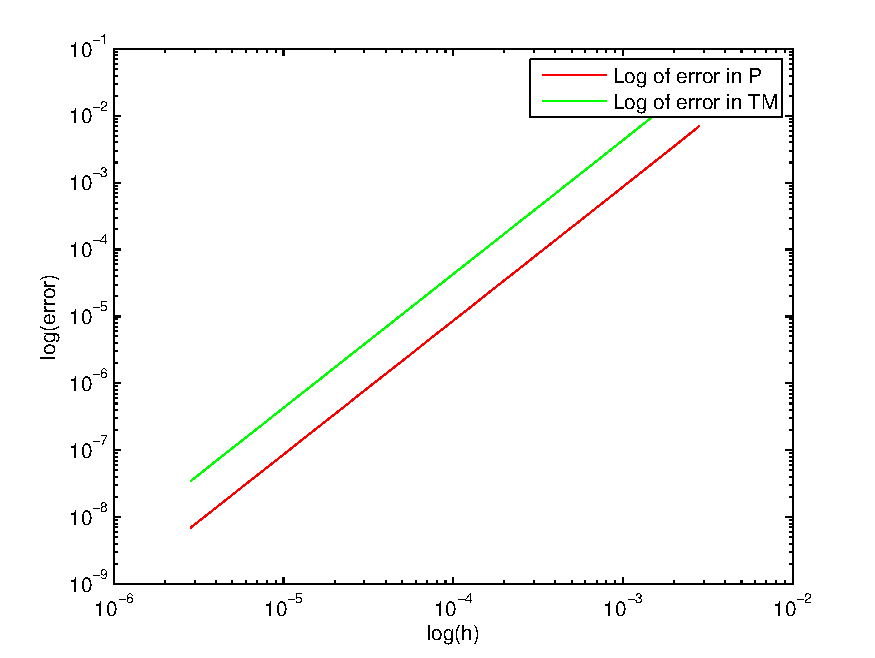
\includegraphics{./img/neoHookConsistency.pdf}
  \caption{Error vs. Perturbation plot for 3D neoHookean
    implementation}
  \label{fig:neoHcon}
\end{figure}
We also calculated the slope of the two error plots numerically. Their
values are in the range from 1.99 to 2.02. Following shows a sample
output for the slopes from the script \texttt{neoHookeanCorrectness.m}
\begin{lstlisting}[frame=single]
  Slope of log(errP) vs log(h) = 2.000e+00 Slope of log(errTM) vs
  log(h) = 2.000e+00
\end{lstlisting}

We tested the plane-stress version of neo-Hookean implementation for
consistency separately. The error in $\mathbf{P}$ has been calculated
using same equation as for the 3-D neo-Hookean implementation. But the
error in tangent modulus is given as
\begin{align*}
  \text{error} =\frac{\underset{\forall \alpha,\beta,\gamma,\delta}{\max}\left(|C^{(h)(2D)}_{\alpha\beta\gamma\delta}-C^{(2D)}_{\alpha\beta\gamma\delta}|\right)}{\underset{\forall i,J,k,L}{\max}\left(C_{\alpha\beta\gamma\delta}\right)}
\end{align*}
This is because $C^{(2D)}_{\alpha\beta\gamma\delta}$ is not merely a
subset of components of $C_{iJkL}$ but requires a correction in order
to be consistent with plane stress condition. The error plot is as
shown in figure \ref{fig:psneoHcon}. As can be seen from the plot and
also verified from numerically calculations, slopes of the error-plots
are always around $2\pm0.02$ Following is a sample slope output from
the script \texttt{planeStressConsistency.m}
\begin{lstlisting}[frame=single]
  Slope of log(errP) vs log(h) = 1.997e+00 Slope of log(errTM) vs
  log(h) = 2.012e+00
\end{lstlisting}
\begin{figure}[h]
  \centering
  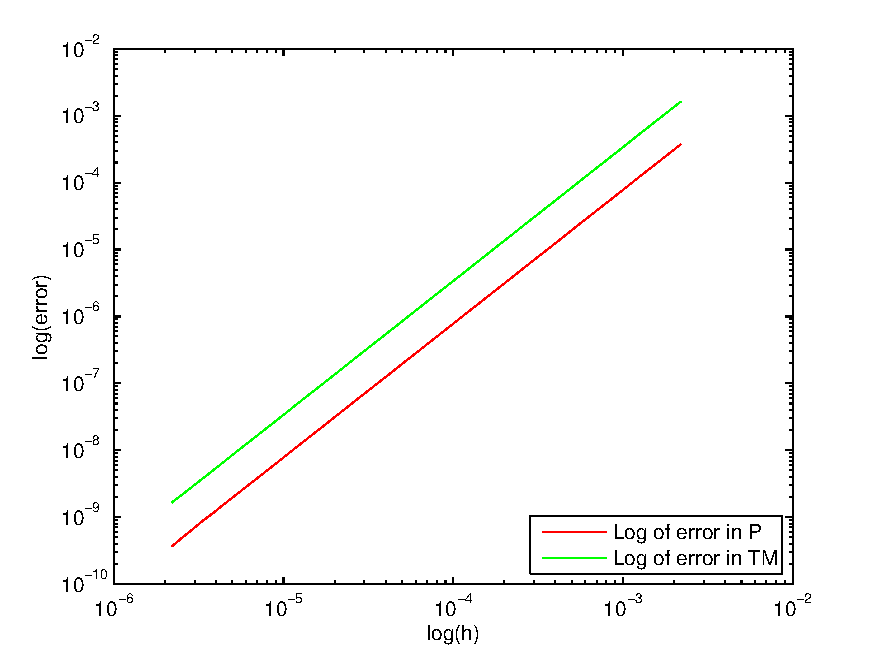
\includegraphics{./img/planeStressConsistency.pdf}
  \caption{Error vs. Perturbation plot for plane stress neoHookean
    implementation}
  \label{fig:psneoHcon}
\end{figure}

\subsubsection{Material Frame Indifference test}
The error in MFI test for $w$ is calculated as
\begin{align*}
  \text{error} = \frac{|w(\mathbf{QF}) - w(\mathbf{F})|}{|w(\mathbf{F})|}
\end{align*}
The error in MFI test for $\mathbf{P}$ is calculated as
\begin{align*}
  \text{error} = \frac{\lVert\mathbf{P}(\mathbf{Q}\mathbf{F}) -\mathbf{Q}\mathbf{P}(\mathbf{F})\rVert}{\lVert\mathbf{Q}\mathbf{P}(\mathbf{F})\rVert}
\end{align*}
The error in $C_{iJkL}$ for MFI test has been calculated as
\begin{align*}
  \text{error} =\frac{\underset{\forall i,J,k,L}{\max}\left(|C_{iJkL}(\mathbf{Q}\mathbf{F})-Q_{ij}Q_{kl}C_{jJlL}(\mathbf{F})|\right)}{\underset{\forall i,J,k,L}{\max}\left(Q_{ij}Q_{kl}C_{jJlL}(\mathbf{F})\right)}
\end{align*}
Following is a sample output for the MFI test from the script
\texttt{neoHookeanCorrectness.m}
\begin{lstlisting}[frame=single]
  Relative error in w due to coordinate rotation = 8.513e-15 Relative
  error in P due to coordinate rotation = 1.65e-14 Relative error in
  TM due to coordinate rotation = 4.359e-14
\end{lstlisting}

\subsubsection{Isotropy Test}
The error in isotropy test for $w$ is calculated as
\begin{align*}
  \text{error} = \frac{|w(\mathbf{FQ}) - w(\mathbf{F})|}{|w(\mathbf{F})|}
\end{align*}
The error in MFI test for $\mathbf{P}$ is calculated as
\begin{align*}
  \text{error} = \frac{\lVert\mathbf{P}(\mathbf{F}\mathbf{Q}) -\mathbf{P}(\mathbf{F})\mathbf{Q}\rVert}{\lVert\mathbf{P}(\mathbf{F})\mathbf{Q}\rVert}
\end{align*}
The error in $C_{iJkL}$ for MFI test has been calculated as
\begin{align*}
  \text{error} =\frac{\underset{\forall i,J,k,L}{\max}\left(|C_{iJkL}(\mathbf{F}\mathbf{Q})-Q_{MJ}Q_{NL}C_{iMkN}(\mathbf{F})|\right)}{\underset{\forall i,J,k,L}{\max}\left(Q_{MJ}Q_{NL}C_{iMkN}(\mathbf{F})\right)}
\end{align*}
The following shows a sample output from the script
\texttt{neoHookeanCorrectness.m}
\begin{lstlisting}[frame=single]
  Relative error in w for symmetry test = 9.222e-15 Relative error in
  P for symmetry test = 2.059e-15 Relative error in TM for symmetry
  test = 3.012e-15
\end{lstlisting}

\subsubsection{Plane Stress Examples}

For both the plane stress examples we have used the material constants
for neoHookean model as follows:
\begin{align*}
  \lambda_0 &= 5\times10^8\\
  \mu_0 & = 1.5\times10^6
\end{align*}
The $F_{11}$ values used are in the closed interval $[0.1,1.5]$. For
both cases, we have plotted the $P_{11}$ and $P_{22}$ components of
$\mathbf{P}$ on the $y$-axis and $F_{11}$ on the $x$-axis.
\begin{itemize}
\item \textbf{Uniaxial deformation}
Figure \ref{fig:uniaxial}, shows the stress-strain curves for uniaxial
deformation.
\begin{figure}[h]
  \centering
  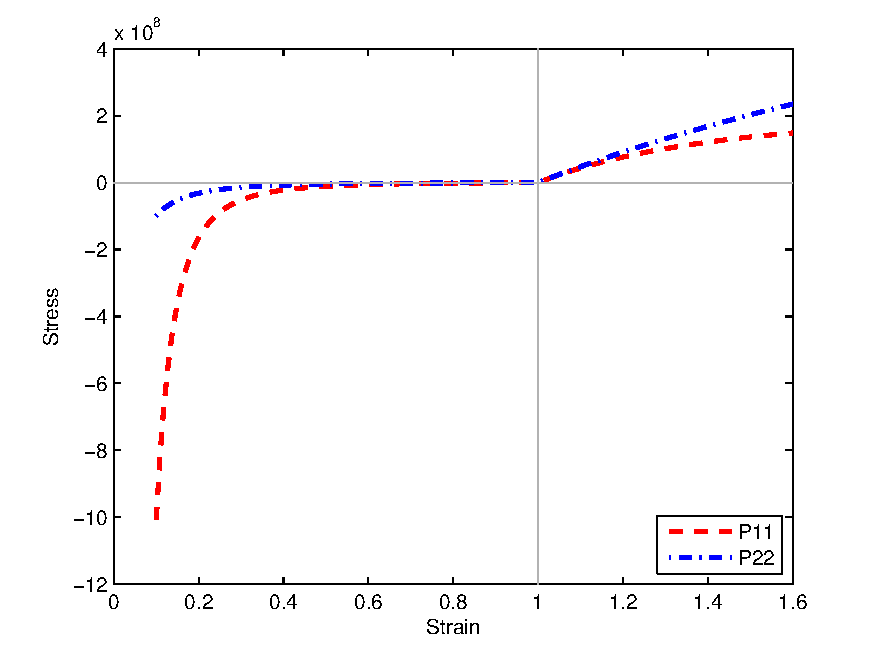
\includegraphics{./img/Uniaxial_1.pdf}
  \caption{Stress vs Strain plot for uniaxial deformation}
  \label{fig:uniaxial}
\end{figure}

\item \textbf{Equibiaxial deformation}
Figure \ref{fig:equibiaxial}, shows the stress-strain curves for
equibiaxial deformation.
\begin{figure}[h]
  \centering
  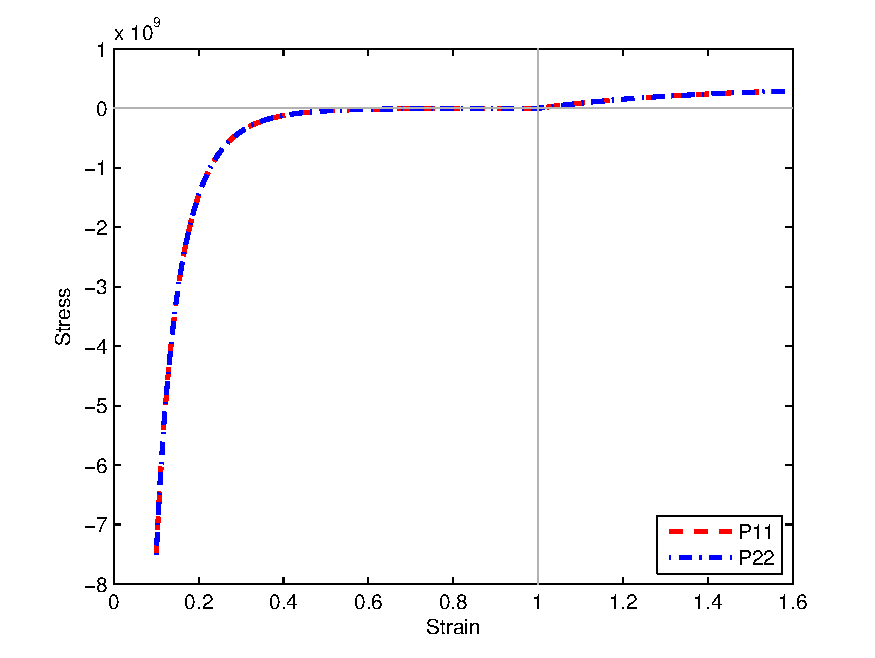
\includegraphics{./img/EquiBiaxial_1.pdf}
  \caption{Stress vs Strain plot for equibiaxial deformation}
  \label{fig:equibiaxial}
\end{figure}
\end{itemize}

\subsection{Discussion and Conclusions}
\subsubsection{Consistency}
For finite difference scheme the values of perturbation $h$ are
assumed to be very small compared to the value of variable $x$ so that
we can use Taylor expansion. But in numerical implementation for
values $h << \sqrt{\epsilon}x$ where $\epsilon$ is machine precision
there is significant amount of rounding error due to floating point
arithmetic. We are generating our arbitrary $\mathbf{F}$ in code as
\begin{lstlisting}[frame=single]
  F = rand(3);
\end{lstlisting}
So components of F belong to the interval $(0,1)$. We are using the
values $h$ as
\begin{align*}
  h = \lVert\mathbf{F}\rVert\times10^{-r}\quad\text{where} r\in(-6,-3)\quad \text{and} r\in\mathbb{Z}
\end{align*}
Thus, we avoid prominent rounding errors in our scheme and obtain a
quadratic scaling as expected. It can be verified from figures
\ref{fig:neoHcon} and \ref{fig:psneoHcon}. Thus, we pass the
consistency requirements.

\subsubsection{MFI and Isotropy}
The errors we calculate in these two tests are relative
errors. Therefore, values closer to $0$ are better. We get values less
than $10^{-13}$. These are very small and close to zero. Thus, we are
sure that our implementation passes these two tests.

\subsection{Plane Stress Examples}
\subsubsection{Uniaxial Deformation}
In this example, we have
\begin{align*}
  \left[F_{\alpha\beta}\right] =   \begin{bmatrix}F_{11} & 0\\ 0 & 1 \end{bmatrix}
\end{align*}
We are constraining the 2-direction to remain undeformed while
1-direction is stretched by ratio $F_{11}$. When $F_{11} < 1$
i.e. compression along direction 1, direction 2 would like to expand
but it is constrained and thus also undergoes compression. Therefore
when $P_{11} < 0$, we expect $P_{22} < 0$. Similar argument is true
for elongation along direction 1. But the magnitudes of the stress
along the two directions are generally not expected to be the same
expect for very small values of $F_{11}$. This trend can be clearly
validated from figure \ref{fig:uniaxial}.

\subsubsection{Equibiaxial Deformation}
In this example, we have
\begin{align*}
  \left[F_{\alpha\beta}\right] =   \begin{bmatrix}F_{11} & 0\\ 0 & F_{11} \end{bmatrix}
\end{align*}
We are imposing same deformation in both 1 and 2 directions. Since the
material is isotropic, we would expect same stress response in both
directions. This is obvious from figure \ref{fig:equibiaxial} where we
find the graph of $P_{11}$ and $P_{22}$ overlapping for all values of
$F_{11}$.

\subsection{Source Code Listing}
The list of files for problem 2 is
\begin{enumerate}
\item \texttt{kronDel.m}: Kronecker-delta function
\item \texttt{neoHookean.m}: 3-D constitutive model. It is a function
  that takes $\mathbf{F},\lambda_0$ and $\mu_0$ as input and gives
  $w,\mathbf{P}$ and $C_{iJkL}$ as output.
\item \texttt{neoHookeanCorrectness.m}:This script tests the 3-D
  neo-Hookean constitutive model for consistency, material frame
  indifference and isotropy.
\item \texttt{planeStressNH.m}: 2-D plane stress neo-Hookean model. It
  is a function that takes $F_{\alpha\beta},\lambda_0$ and $\mu_0$ as
  input and gives $w,P_{\alpha\beta}$ and
  $C^{(2D)}_{\alpha\beta\gamma\delta}$ as output.
\item \texttt{planeStressConsistency.m}:This script tests the 2-D
  plane stress neoHookean model for consistency.
\item \texttt{planeStressExamples.m}:This script implements the
  uniaxial deformation and equibiaxial deformation examples for
  plane-stress.
\end{enumerate}


\end{document}
